\documentclass[11pt]{article}
\usepackage[margin=1in]{geometry}
\usepackage{amsmath,amssymb,amsthm}
\usepackage{microtype}
\usepackage{enumitem}
\setlist{nosep,leftmargin=*}
\usepackage{booktabs}
\usepackage{xurl}
\usepackage{tikz}
\usepackage[colorlinks=true,allcolors=blue]{hyperref}
\sloppy
\newtheorem{theorem}{Theorem}
\newtheorem{lemma}[theorem]{Lemma}
\newtheorem{corollary}[theorem]{Corollary}
\theoremstyle{definition}
\newtheorem{definition}[theorem]{Definition}
\theoremstyle{remark}
\newtheorem{remark}[theorem]{Remark}
\setlength{\parskip}{0.3em}
\title{The pinwheel tilings have no undecorated local rules}
\author{John Cullen\thanks{Draft of 8 November 2026, prepared with Claude
(Anthropic). The results come from proofs with executable checks in the
public repository \url{https://github.com/jscul/knotlab}; Section~\ref{sec:evidence}
lists them, and \texttt{replay.py}, written separately from them, recomputes the
headline facts. No human expert has reviewed this note.}}
\date{}
\begin{document}
\maketitle

\begin{abstract}
Radin forced the pinwheel tilings of the plane by matching rules on decorated
tiles. We show that decorations cannot be dropped: for every radius $r$ there is
a periodic tiling by the pinwheel triangle in which every patch of radius $r$ is
a patch of a pinwheel tiling. The witness is explicit. Four triangles around a
common right angle form a rhombus; the lattice tiling by these rhombi, cut once
by Conway's subdivision, already has every \emph{collar} (a tile with all the
tiles it touches) equal to a collar of a pinwheel tiling, and each further cut
defeats a larger radius. The collar rule does force one level of the hierarchy,
and no more. Hidden labels that are read from a bounded window of the tiling do
not help either, and of the 1{,}024 ways a decorated substitution can place one
hidden bit on each tile, 1{,}022 still admit a periodic tiling at every radius.
\end{abstract}

\section{Introduction}

The pinwheel tilings \cite{Rad94} are the tilings of the plane by copies of the
right triangle with legs $1$ and $2$ in which every finite patch occurs in an
iterate of Conway's subdivision of one triangle into five. They are
non-periodic, and their tiles point in infinitely many directions, uniformly
distributed. Radin showed that they are the tilings allowed by finitely many
\emph{decorated} tiles with matching rules; Mozes \cite{Moz89} and
Goodman-Strauss \cite{GS98} extended this to substitution tilings in general.

A tiling space has \emph{local rules} of radius $r$ in Levitov's sense
\cite{Lev88} if a tiling belongs to it as soon as each of its patches of radius
$r$ occurs in some tiling of the space. Undecorated local rules exist for some
quasiperiodic rhombus tilings and fail for others \cite{Lev88,Soc90}. For the
pinwheel the question does not seem to be settled in print. We answer it.

\begin{theorem}\label{thm:main}
For every $r\ge 1$ there is a periodic tiling of the plane by the pinwheel
triangle all of whose patches of tile radius $r$ are congruent, after scaling,
to patches of pinwheel tilings. Hence the pinwheel tilings have no undecorated
local rules of any radius.
\end{theorem}

The tilings in Theorem~\ref{thm:main} are cuts of one simple crystal
(Figure~\ref{fig:rhombus}), which shows how the hierarchy hides a crystal's
seams.

\section{Tiles, cuts and collars}

A tile is a triple $(O,P,Q)$: the right angle, the end of the long leg and the
end of the short leg of a right triangle with legs $|OQ|=1$ and $|OP|=2$.
Conway's cut adds the points
\[
H=\tfrac{4Q+P}{5},\quad M=\tfrac{O+P}{2},\quad F_1=\tfrac{O+H}{2},\quad F_2=\tfrac{H+P}{2}
\]
and replaces the tile by its five children
$(H,O,Q)$, $(F_1,M,O)$, $(F_1,M,H)$, $(F_2,H,M)$ and $(F_2,P,M)$, each similar
to it with ratio $1/\sqrt5$. The cut of a tiling cuts every tile.

The \emph{collar} of a tile is the tile together with every tile that shares a
point with it, recorded in the tile's own affine frame ($O$ at $0$, $Q$ at
$(1,0)$, $P$ at $(0,1)$) together with its handedness. A collar is
\emph{complete} when it covers a neighbourhood of its tile. Collared tiles
closed under a substitution describe its tiling space \cite{AP98}, and for the
pinwheel this was done in \cite{BDHS10,FWW14}. Starting from one triangle and
closing under the cut gives 193 collars, of which 108 are complete
\cite{CP-atlas}; the complete ones are exactly the collars of tiles of pinwheel
tilings. A tiling is \emph{collar-legal} if every collar is
one of these 108.

\begin{lemma}\label{lem:cut}
The cut maps every complete pinwheel collar to five complete pinwheel collars.
So the cut of a collar-legal tiling is collar-legal.
\end{lemma}

\begin{proof}
Children that touch have parents that touch, so a child's collar is computed in
the cut of its parent's collar; the set of 193 collars is closed under this map,
and a child of a tile whose collar covers a neighbourhood of it has a collar
covering a neighbourhood of the child.
\end{proof}

\section{A periodic plane that obeys the collar rule}

\begin{figure}[t]
\centering
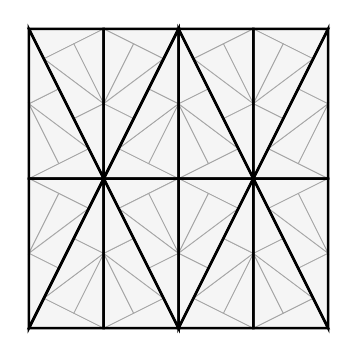
\begin{tikzpicture}[scale=0.95]
\draw[gray!70, line width=0.3pt, fill=gray!8] (-1.200,0.400) -- (-2.000,0.000) -- (-1.000,0.000) -- cycle;
\draw[gray!70, line width=0.3pt, fill=gray!8] (-1.600,0.200) -- (-2.000,1.000) -- (-2.000,0.000) -- cycle;
\draw[gray!70, line width=0.3pt, fill=gray!8] (-1.600,0.200) -- (-2.000,1.000) -- (-1.200,0.400) -- cycle;
\draw[gray!70, line width=0.3pt, fill=gray!8] (-1.600,1.200) -- (-1.200,0.400) -- (-2.000,1.000) -- cycle;
\draw[gray!70, line width=0.3pt, fill=gray!8] (-1.600,1.200) -- (-2.000,2.000) -- (-2.000,1.000) -- cycle;
\draw[gray!70, line width=0.3pt, fill=gray!8] (-1.200,-0.400) -- (-2.000,0.000) -- (-1.000,0.000) -- cycle;
\draw[gray!70, line width=0.3pt, fill=gray!8] (-1.600,-0.200) -- (-2.000,-1.000) -- (-2.000,0.000) -- cycle;
\draw[gray!70, line width=0.3pt, fill=gray!8] (-1.600,-0.200) -- (-2.000,-1.000) -- (-1.200,-0.400) -- cycle;
\draw[gray!70, line width=0.3pt, fill=gray!8] (-1.600,-1.200) -- (-1.200,-0.400) -- (-2.000,-1.000) -- cycle;
\draw[gray!70, line width=0.3pt, fill=gray!8] (-1.600,-1.200) -- (-2.000,-2.000) -- (-2.000,-1.000) -- cycle;
\draw[gray!70, line width=0.3pt, fill=gray!8] (-0.200,-1.600) -- (-1.000,-2.000) -- (0.000,-2.000) -- cycle;
\draw[gray!70, line width=0.3pt, fill=gray!8] (-0.600,-1.800) -- (-1.000,-1.000) -- (-1.000,-2.000) -- cycle;
\draw[gray!70, line width=0.3pt, fill=gray!8] (-0.600,-1.800) -- (-1.000,-1.000) -- (-0.200,-1.600) -- cycle;
\draw[gray!70, line width=0.3pt, fill=gray!8] (-0.600,-0.800) -- (-0.200,-1.600) -- (-1.000,-1.000) -- cycle;
\draw[gray!70, line width=0.3pt, fill=gray!8] (-0.600,-0.800) -- (-1.000,0.000) -- (-1.000,-1.000) -- cycle;
\draw[gray!70, line width=0.3pt, fill=gray!8] (-1.800,-1.600) -- (-1.000,-2.000) -- (-2.000,-2.000) -- cycle;
\draw[gray!70, line width=0.3pt, fill=gray!8] (-1.400,-1.800) -- (-1.000,-1.000) -- (-1.000,-2.000) -- cycle;
\draw[gray!70, line width=0.3pt, fill=gray!8] (-1.400,-1.800) -- (-1.000,-1.000) -- (-1.800,-1.600) -- cycle;
\draw[gray!70, line width=0.3pt, fill=gray!8] (-1.400,-0.800) -- (-1.800,-1.600) -- (-1.000,-1.000) -- cycle;
\draw[gray!70, line width=0.3pt, fill=gray!8] (-1.400,-0.800) -- (-1.000,0.000) -- (-1.000,-1.000) -- cycle;
\draw[gray!70, line width=0.3pt, fill=gray!8] (-0.200,1.600) -- (-1.000,2.000) -- (0.000,2.000) -- cycle;
\draw[gray!70, line width=0.3pt, fill=gray!8] (-0.600,1.800) -- (-1.000,1.000) -- (-1.000,2.000) -- cycle;
\draw[gray!70, line width=0.3pt, fill=gray!8] (-0.600,1.800) -- (-1.000,1.000) -- (-0.200,1.600) -- cycle;
\draw[gray!70, line width=0.3pt, fill=gray!8] (-0.600,0.800) -- (-0.200,1.600) -- (-1.000,1.000) -- cycle;
\draw[gray!70, line width=0.3pt, fill=gray!8] (-0.600,0.800) -- (-1.000,0.000) -- (-1.000,1.000) -- cycle;
\draw[gray!70, line width=0.3pt, fill=gray!8] (-1.800,1.600) -- (-1.000,2.000) -- (-2.000,2.000) -- cycle;
\draw[gray!70, line width=0.3pt, fill=gray!8] (-1.400,1.800) -- (-1.000,1.000) -- (-1.000,2.000) -- cycle;
\draw[gray!70, line width=0.3pt, fill=gray!8] (-1.400,1.800) -- (-1.000,1.000) -- (-1.800,1.600) -- cycle;
\draw[gray!70, line width=0.3pt, fill=gray!8] (-1.400,0.800) -- (-1.800,1.600) -- (-1.000,1.000) -- cycle;
\draw[gray!70, line width=0.3pt, fill=gray!8] (-1.400,0.800) -- (-1.000,0.000) -- (-1.000,1.000) -- cycle;
\draw[gray!70, line width=0.3pt, fill=gray!8] (0.800,0.400) -- (0.000,0.000) -- (1.000,0.000) -- cycle;
\draw[gray!70, line width=0.3pt, fill=gray!8] (0.400,0.200) -- (0.000,1.000) -- (0.000,0.000) -- cycle;
\draw[gray!70, line width=0.3pt, fill=gray!8] (0.400,0.200) -- (0.000,1.000) -- (0.800,0.400) -- cycle;
\draw[gray!70, line width=0.3pt, fill=gray!8] (0.400,1.200) -- (0.800,0.400) -- (0.000,1.000) -- cycle;
\draw[gray!70, line width=0.3pt, fill=gray!8] (0.400,1.200) -- (0.000,2.000) -- (0.000,1.000) -- cycle;
\draw[gray!70, line width=0.3pt, fill=gray!8] (-0.800,0.400) -- (0.000,0.000) -- (-1.000,0.000) -- cycle;
\draw[gray!70, line width=0.3pt, fill=gray!8] (-0.400,0.200) -- (0.000,1.000) -- (0.000,0.000) -- cycle;
\draw[gray!70, line width=0.3pt, fill=gray!8] (-0.400,0.200) -- (0.000,1.000) -- (-0.800,0.400) -- cycle;
\draw[gray!70, line width=0.3pt, fill=gray!8] (-0.400,1.200) -- (-0.800,0.400) -- (0.000,1.000) -- cycle;
\draw[gray!70, line width=0.3pt, fill=gray!8] (-0.400,1.200) -- (0.000,2.000) -- (0.000,1.000) -- cycle;
\draw[gray!70, line width=0.3pt, fill=gray!8] (0.800,-0.400) -- (0.000,0.000) -- (1.000,0.000) -- cycle;
\draw[gray!70, line width=0.3pt, fill=gray!8] (0.400,-0.200) -- (0.000,-1.000) -- (0.000,0.000) -- cycle;
\draw[gray!70, line width=0.3pt, fill=gray!8] (0.400,-0.200) -- (0.000,-1.000) -- (0.800,-0.400) -- cycle;
\draw[gray!70, line width=0.3pt, fill=gray!8] (0.400,-1.200) -- (0.800,-0.400) -- (0.000,-1.000) -- cycle;
\draw[gray!70, line width=0.3pt, fill=gray!8] (0.400,-1.200) -- (0.000,-2.000) -- (0.000,-1.000) -- cycle;
\draw[gray!70, line width=0.3pt, fill=gray!8] (-0.800,-0.400) -- (0.000,0.000) -- (-1.000,0.000) -- cycle;
\draw[gray!70, line width=0.3pt, fill=gray!8] (-0.400,-0.200) -- (0.000,-1.000) -- (0.000,0.000) -- cycle;
\draw[gray!70, line width=0.3pt, fill=gray!8] (-0.400,-0.200) -- (0.000,-1.000) -- (-0.800,-0.400) -- cycle;
\draw[gray!70, line width=0.3pt, fill=gray!8] (-0.400,-1.200) -- (-0.800,-0.400) -- (0.000,-1.000) -- cycle;
\draw[gray!70, line width=0.3pt, fill=gray!8] (-0.400,-1.200) -- (0.000,-2.000) -- (0.000,-1.000) -- cycle;
\draw[gray!70, line width=0.3pt, fill=gray!8] (1.800,-1.600) -- (1.000,-2.000) -- (2.000,-2.000) -- cycle;
\draw[gray!70, line width=0.3pt, fill=gray!8] (1.400,-1.800) -- (1.000,-1.000) -- (1.000,-2.000) -- cycle;
\draw[gray!70, line width=0.3pt, fill=gray!8] (1.400,-1.800) -- (1.000,-1.000) -- (1.800,-1.600) -- cycle;
\draw[gray!70, line width=0.3pt, fill=gray!8] (1.400,-0.800) -- (1.800,-1.600) -- (1.000,-1.000) -- cycle;
\draw[gray!70, line width=0.3pt, fill=gray!8] (1.400,-0.800) -- (1.000,0.000) -- (1.000,-1.000) -- cycle;
\draw[gray!70, line width=0.3pt, fill=gray!8] (0.200,-1.600) -- (1.000,-2.000) -- (0.000,-2.000) -- cycle;
\draw[gray!70, line width=0.3pt, fill=gray!8] (0.600,-1.800) -- (1.000,-1.000) -- (1.000,-2.000) -- cycle;
\draw[gray!70, line width=0.3pt, fill=gray!8] (0.600,-1.800) -- (1.000,-1.000) -- (0.200,-1.600) -- cycle;
\draw[gray!70, line width=0.3pt, fill=gray!8] (0.600,-0.800) -- (0.200,-1.600) -- (1.000,-1.000) -- cycle;
\draw[gray!70, line width=0.3pt, fill=gray!8] (0.600,-0.800) -- (1.000,0.000) -- (1.000,-1.000) -- cycle;
\draw[gray!70, line width=0.3pt, fill=gray!8] (1.800,1.600) -- (1.000,2.000) -- (2.000,2.000) -- cycle;
\draw[gray!70, line width=0.3pt, fill=gray!8] (1.400,1.800) -- (1.000,1.000) -- (1.000,2.000) -- cycle;
\draw[gray!70, line width=0.3pt, fill=gray!8] (1.400,1.800) -- (1.000,1.000) -- (1.800,1.600) -- cycle;
\draw[gray!70, line width=0.3pt, fill=gray!8] (1.400,0.800) -- (1.800,1.600) -- (1.000,1.000) -- cycle;
\draw[gray!70, line width=0.3pt, fill=gray!8] (1.400,0.800) -- (1.000,0.000) -- (1.000,1.000) -- cycle;
\draw[gray!70, line width=0.3pt, fill=gray!8] (0.200,1.600) -- (1.000,2.000) -- (0.000,2.000) -- cycle;
\draw[gray!70, line width=0.3pt, fill=gray!8] (0.600,1.800) -- (1.000,1.000) -- (1.000,2.000) -- cycle;
\draw[gray!70, line width=0.3pt, fill=gray!8] (0.600,1.800) -- (1.000,1.000) -- (0.200,1.600) -- cycle;
\draw[gray!70, line width=0.3pt, fill=gray!8] (0.600,0.800) -- (0.200,1.600) -- (1.000,1.000) -- cycle;
\draw[gray!70, line width=0.3pt, fill=gray!8] (0.600,0.800) -- (1.000,0.000) -- (1.000,1.000) -- cycle;
\draw[gray!70, line width=0.3pt, fill=gray!8] (1.200,0.400) -- (2.000,0.000) -- (1.000,0.000) -- cycle;
\draw[gray!70, line width=0.3pt, fill=gray!8] (1.600,0.200) -- (2.000,1.000) -- (2.000,0.000) -- cycle;
\draw[gray!70, line width=0.3pt, fill=gray!8] (1.600,0.200) -- (2.000,1.000) -- (1.200,0.400) -- cycle;
\draw[gray!70, line width=0.3pt, fill=gray!8] (1.600,1.200) -- (1.200,0.400) -- (2.000,1.000) -- cycle;
\draw[gray!70, line width=0.3pt, fill=gray!8] (1.600,1.200) -- (2.000,2.000) -- (2.000,1.000) -- cycle;
\draw[gray!70, line width=0.3pt, fill=gray!8] (1.200,-0.400) -- (2.000,0.000) -- (1.000,0.000) -- cycle;
\draw[gray!70, line width=0.3pt, fill=gray!8] (1.600,-0.200) -- (2.000,-1.000) -- (2.000,0.000) -- cycle;
\draw[gray!70, line width=0.3pt, fill=gray!8] (1.600,-0.200) -- (2.000,-1.000) -- (1.200,-0.400) -- cycle;
\draw[gray!70, line width=0.3pt, fill=gray!8] (1.600,-1.200) -- (1.200,-0.400) -- (2.000,-1.000) -- cycle;
\draw[gray!70, line width=0.3pt, fill=gray!8] (1.600,-1.200) -- (2.000,-2.000) -- (2.000,-1.000) -- cycle;
\draw[black, line width=0.9pt] (-2.000,0.000) -- (-2.000,2.000) -- (-1.000,0.000) -- cycle;
\draw[black, line width=0.9pt] (-2.000,0.000) -- (-2.000,-2.000) -- (-1.000,0.000) -- cycle;
\draw[black, line width=0.9pt] (-1.000,-2.000) -- (-1.000,0.000) -- (0.000,-2.000) -- cycle;
\draw[black, line width=0.9pt] (-1.000,-2.000) -- (-1.000,0.000) -- (-2.000,-2.000) -- cycle;
\draw[black, line width=0.9pt] (-1.000,2.000) -- (-1.000,0.000) -- (0.000,2.000) -- cycle;
\draw[black, line width=0.9pt] (-1.000,2.000) -- (-1.000,0.000) -- (-2.000,2.000) -- cycle;
\draw[black, line width=0.9pt] (0.000,0.000) -- (0.000,2.000) -- (1.000,0.000) -- cycle;
\draw[black, line width=0.9pt] (0.000,0.000) -- (0.000,2.000) -- (-1.000,0.000) -- cycle;
\draw[black, line width=0.9pt] (0.000,0.000) -- (0.000,-2.000) -- (1.000,0.000) -- cycle;
\draw[black, line width=0.9pt] (0.000,0.000) -- (0.000,-2.000) -- (-1.000,0.000) -- cycle;
\draw[black, line width=0.9pt] (1.000,-2.000) -- (1.000,0.000) -- (2.000,-2.000) -- cycle;
\draw[black, line width=0.9pt] (1.000,-2.000) -- (1.000,0.000) -- (0.000,-2.000) -- cycle;
\draw[black, line width=0.9pt] (1.000,2.000) -- (1.000,0.000) -- (2.000,2.000) -- cycle;
\draw[black, line width=0.9pt] (1.000,2.000) -- (1.000,0.000) -- (0.000,2.000) -- cycle;
\draw[black, line width=0.9pt] (2.000,0.000) -- (2.000,2.000) -- (1.000,0.000) -- cycle;
\draw[black, line width=0.9pt] (2.000,0.000) -- (2.000,-2.000) -- (1.000,0.000) -- cycle;
\end{tikzpicture}

\caption{The rhombus lattice (thick) and its cut (thin). Every one of the 20
tiles in a period of the cut has a pinwheel collar.}
\label{fig:rhombus}
\end{figure}

Let $R$ be the tiling by the four tiles $\big((0,0),(0,\pm2),(\pm1,0)\big)$,
which form a rhombus with diagonals $2$ and $4$, and their translates by the
lattice $\Lambda=\mathbb{Z}(1,2)+\mathbb{Z}(1,-2)$. Let $R_k$ be its $k$-fold
cut.

\begin{theorem}\label{thm:witness}
$R_1$ is a $\Lambda$-periodic tiling with $20$ tiles per period in which every
collar is a complete pinwheel collar. It uses ten of the 108.
\end{theorem}

\begin{proof}
The central rhombus is a fundamental domain of $\Lambda$, so its cut contains
one tile of every orbit, and a collar is invariant under translation. The
twenty collars are computed exactly.
\end{proof}

$R$ itself is not collar-legal: four right angles meet at the centre of each
rhombus, which never happens in a pinwheel tiling. Most of the crystals tested
in \cite{CP-atlas} stay illegal after cutting; the rectangle lattice, for
instance, fails after one and after two cuts. But $R$ is not alone. Among the
domino tilings of small tori with diagonals, brick rows with diagonals of period
four are collar-legal after one cut, and further planes after two cuts.

\begin{theorem}\label{thm:radius}
Let $w>0$ be the least distance, over the 108 complete collars, from the
central tile to the outside of the collar (for legs $1$ and $2$,
$w\approx 0.447$). If $T$ is collar-legal and $(r+1)\sqrt5\,5^{-k/2}<w$, then
every patch of tile radius $r$ of the $k$-fold cut of $T$ is congruent, after
scaling, to a patch of a pinwheel tiling.
\end{theorem}

\begin{proof}
Let $d$ be a tile of the cut and $c$ the tile of $T$ containing it. A tile
reached from $d$ in at most $r$ steps between touching tiles lies within
$r\sqrt5\,5^{-k/2}$ of $c$, hence inside the union of $c$'s collar. There the
$k$-fold cut of $T$ is the $k$-fold cut of that collar, which is a pinwheel
collar, and the $k$-fold cut of a pinwheel patch is a pinwheel patch.
\end{proof}

Theorem~\ref{thm:main} follows from Theorems~\ref{thm:witness} and
\ref{thm:radius} with Lemma~\ref{lem:cut}: $R_k$ is periodic for every $k$. The
bound is far from sharp. $R_2$ (100 tiles per period) already passes the
complete list of 1{,}168 radius-2 neighbourhoods of the pinwheel's planar map,
and $R_3$ the list of 3{,}530 radius-3 neighbourhoods.

\section{One level of the hierarchy is forced, and no more}

\begin{theorem}\label{thm:compose}
In every collar-legal tiling of the plane, each tile's collar determines its
parent (which child of which larger triangle it is), and touching tiles that
should be siblings determine the same parent. So every collar-legal tiling is
the cut of a tiling by triangles $\sqrt5$ times larger.
\end{theorem}

The larger tiling need not be collar-legal. Its collars satisfy only the weaker
condition that their cut is collar-legal; there are 1{,}264 such collars for
each handedness, 54 of them pinwheel collars, and 156 survive arc consistency.
The rhombus collar is one of the survivors, which is how $R_1$ escapes.

\section{Hidden labels}

Matching rules carry hidden information. How much is needed?

\begin{lemma}\label{lem:local}
If each hidden label is a function of a bounded window of the undecorated
tiling, then for every radius the labelled local rule admits a periodic tiling:
$R_k$, labelled by the same function, for $k$ large.
\end{lemma}

\begin{proof}
Every patch of radius $r+\rho$ of $R_k$ is a pinwheel patch for $k$ large, and
the labels within radius $r$ are read from it.
\end{proof}

In particular a tile's child index, or any finite part of its address in the
hierarchy, is useless as a decoration. Every known decoration is a
\emph{decorated substitution}: the cut gives each child a label determined by
its parent's label and its child index. For these, a crystal admitted by the
labelled collar rule is admitted by the labelled rule of every radius after
more cuts, so the collar rule is the right test.

\begin{theorem}\label{thm:onebit}
Of the 1{,}024 decorated substitutions on two labels, 1{,}022 admit a periodic
plane: a cut crystal with a periodic labelling obeying the labelled collar rule.
The remaining decoration, with child labels $1\,0\,1\,0\,1$ for a parent
labelled $0$ and $0\,0\,1\,1\,0$ for a parent labelled $1$ (and the same with
the labels exchanged), excludes every crystal tried; in it every parent's label
is forced, but a joint consistency test leaves labelled parent collars that are
not collars of the rule, so it is not known whether it forces the pinwheel.
\end{theorem}

The crystals used are the rhombus lattice, brick rows of $1\times2$ rectangles
with two families of diagonal patterns, and eleven domino tilings of tori up to
$4\times4$. One mixed tiling of the $4\times4$ torus, with dominoes in both
directions, defeats six of the decorations that survive the simpler crystals.

\paragraph{Question.} Does the last decoration force the pinwheel? If it does,
one hidden bit per tile suffices to force the pinwheel tilings.

\section{Evidence}\label{sec:evidence}

Every statement above is proved by hand with finite computations checked in
the repository \url{https://github.com/jscul/knotlab}:
\begin{itemize}
\item the 108 collars and the radius-2 list:
\texttt{proofs/PINWHEEL-ATLAS-20261107-001A};
\item Theorems~\ref{thm:witness} and \ref{thm:radius}:
\texttt{proofs/COLLAR-PLANE-20261108-001A}, with the radius-3 test in
\texttt{research/COLLAR-PLANE-20261108-001};
\item Theorem~\ref{thm:compose}: \texttt{proofs/COLLAR-PLANE-20261108-001B};
\item the census of crystals: \texttt{artifacts/COLLAR-PLANE-20261108-001C};
\item Lemma~\ref{lem:local} and Theorem~\ref{thm:onebit}:
\texttt{proofs/ROUND-PRICE-20261108-001A}, \texttt{proofs/ROUND-PRICE-20261108-001B},
\texttt{proofs/ONE-BIT-20261108-001A} and
\texttt{artifacts/ONE-BIT-20261108-001B}.
\end{itemize}
The script \texttt{replay.py} beside this note recomputes, with its own code and
a different completeness test (an angle count), the 193 collars and the 108
complete ones, Lemma~\ref{lem:cut}, and Theorem~\ref{thm:witness} for $R_1$
and $R_2$, with the uncut rhombus lattice and the cut rectangle lattice as
controls.

\begin{thebibliography}{99}
\bibitem{AP98} J.~E.~Anderson and I.~F.~Putnam, \emph{Topological invariants
for substitution tilings and their associated C$^*$-algebras}, Ergodic Theory
Dynam. Systems 18 (1998), 509--537.
\bibitem{BDHS10} M.~Barge, B.~Diamond, J.~Hunton and L.~Sadun, \emph{Cohomology
of substitution tiling spaces}, Ergodic Theory Dynam. Systems 30 (2010),
1607--1627.
\bibitem{CP-atlas} J.~Cullen, \emph{The pinwheel's own law}, knotlab record
\texttt{PINWHEEL-ATLAS-20261107-001} (2026).
\bibitem{DS95} S.~Dworkin and J.-I.~Shieh, \emph{Deceptions in quasicrystal
growth}, Comm. Math. Phys. 168 (1995), 337--352.
\bibitem{FWW14} D.~Frettl\"oh, B.~Whitehead and M.~Whittaker, \emph{Cohomology
of the pinwheel tiling}, J. Aust. Math. Soc. 97 (2014), 162--179.
\bibitem{GS98} C.~Goodman-Strauss, \emph{Matching rules and substitution
tilings}, Ann. of Math. 147 (1998), 181--223.
\bibitem{JR21} E.~Jeandel and M.~Rao, \emph{An aperiodic set of 11 Wang tiles},
Adv. Comb. (2021).
\bibitem{Lev88} L.~S.~Levitov, \emph{Local rules for quasicrystals}, Comm.
Math. Phys. 119 (1988), 627--666.
\bibitem{Moz89} S.~Mozes, \emph{Tilings, substitution systems and dynamical
systems generated by them}, J. Analyse Math. 53 (1989), 139--186.
\bibitem{Rad94} C.~Radin, \emph{The pinwheel tilings of the plane}, Ann. of
Math. 139 (1994), 661--702.
\bibitem{Soc90} J.~E.~S.~Socolar, \emph{Weak matching rules for
quasicrystals}, Comm. Math. Phys. 129 (1990), 599--619.
\bibitem{Sol98} B.~Solomyak, \emph{Nonperiodicity implies unique composition
for self-similar translationally finite tilings}, Discrete Comput. Geom. 20
(1998), 265--279.
\end{thebibliography}

\end{document}
